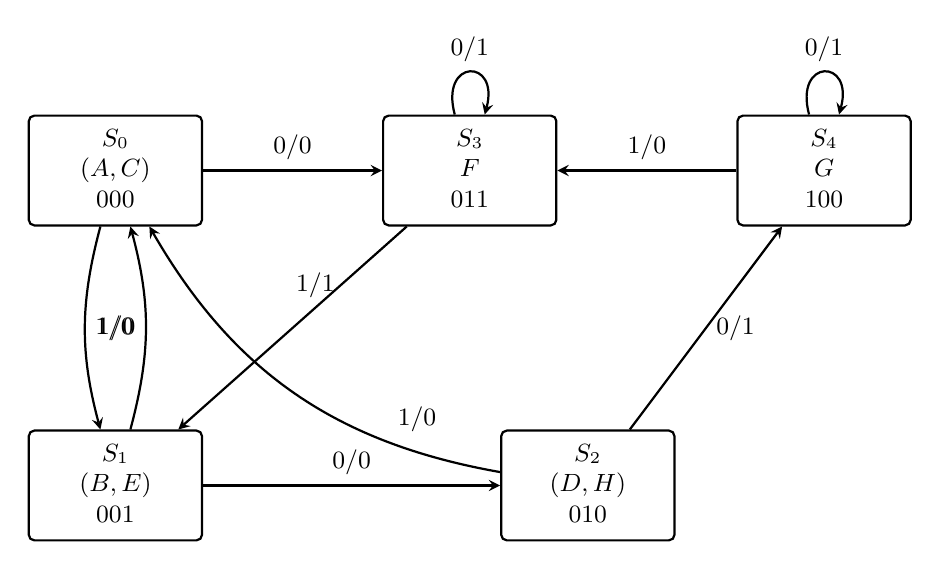
\begin{tikzpicture}[
    >=stealth,
    every node/.style={font=\small},
    state/.style={
        draw, rectangle, rounded corners=2pt, thick,
        align=center, minimum width=2.2cm,
        minimum height=1.1cm
    },
    every edge/.style={draw, thick, ->}
]
% Nodes positioning matching the handwritten layout using tabular for safe multi-line text
\node[state] (S0) at (0, 4) {\begin{tabular}{c} $S_0$ \\ $(A,C)$ \\ $000$ \end{tabular}};
\node[state] (S3) at (4.5, 4) {\begin{tabular}{c} $S_3$ \\ $F$ \\ $011$ \end{tabular}};
\node[state] (S4) at (9, 4) {\begin{tabular}{c} $S_4$ \\ $G$ \\ $100$ \end{tabular}};

\node[state] (S1) at (0, 0) {\begin{tabular}{c} $S_1$ \\ $(B,E)$ \\ $001$ \end{tabular}};
\node[state] (S2) at (6, 0) {\begin{tabular}{c} $S_2$ \\ $(D,H)$ \\ $010$ \end{tabular}};

% Transitions

% S0 <-> S1
\draw (S0) edge[bend right=15] node[right] {$1/0$} (S1);
\draw (S1) edge[bend right=15] node[left] {$1/0$} (S0);

% S0 -> S3
\draw (S0) edge node[above] {$0/0$} (S3);

% S1 -> S2
\draw (S1) edge node[above] {$0/0$} (S2);

% S2 -> S0 
\draw (S2) edge[bend left=25] node[above right, pos=0.25] {$1/0$} (S0);

% S3 -> S1
\draw (S3) edge node[above, pos=0.4] {$1/1$} (S1);

% S2 -> S4
\draw (S2) edge node[right, pos=0.5] {$0/1$} (S4);

% S4 -> S3
\draw (S4) edge node[above] {$1/0$} (S3);

% Self-loop S3 (Above)
\draw (S3) edge[loop above, looseness=5] node[above] {$0/1$} (S3);

% Self-loop S4 (Above)
\draw (S4) edge[loop above, looseness=5] node[above] {$0/1$} (S4);

\end{tikzpicture}
